\vspace{10mm} %5mm vertical space
 
\vfill

\section{ Introduction }

\hspace{2cm} By virtue of nature, human needs many necessary and secondary requests everyday such as medicines, food, clothes, books and others which leading to the emergence of the concept of delivery. The delivery process helps the person who request something to get his request quickly and without any effort to his location wherever he locates. We can define delivery as the process of transporting goods from a source location to a predefined destination. 
To deliver the order to the requester, the order is not transferring from the hub to the requester location directly, it is following a trajectory starting from the hub then to the market and end at the final destination.
\par
Order-to-Delivery is a common term in the automotive business. The concept of OTD process is relatively consistent within the automotive industry even if the process can be described in different levels of detail.
Order-to-Delivery is a process that flows over multiple different functions within an organization. It can be considered one of the most critical processes within logistics. The flow starts when a customer places an order and ends with the customer receiving a finished goods or services. To realize this, there are certain sub-processes that need to be fulfilled. The starting processes can be tracked back to the recognition of a need at the customer. This recognition will lead to an order placement with the supplier, i.e. the manufacturer. After the order is placed, the supplier performs the necessary actions to fulfil the order and provide the finished goods. Here the transportation process takes place, when the finished goods is picked up at the supplier until it is delivered at the customer or other delivery address. The last set of sub-processes consist of making the goods available to use after delivery to costumer.
\par According to Jonsson and Mattson (2016) the Order-to-Deliver can in short be described as the following steps:

\begin{itemize}
    \item Order reception from customer 
    \item Order handling 
    \item Finishing of ordered goods
    \item Internal transportation of goods
    \item Packaging and loading
    \item Transportation
    \item Billing
\end{itemize}

\par Supply chain management and E-commerce are communities in which the delivery process is an important part of them. Supply chain management has many definitions, some of these definitions stated below give a general understanding of the subject.
\par" 
\textbf{A supply chain is the set of entities that are involved in the design of new products and services, procuring raw materials, transforming them into semi-finished and finished products, and delivering them to the end customers}” (Swaminathan, 2001)
\par "
\textbf {A supply chain is a network of partners who collectively convert a basic commodity (upstream) into a finished product (downstream) that is valued by end-customers, and who manage returns at each stage} " (Alan Harrison, 2014) 
\par"
\textbf{The integration of business processes from end user through original suppliers that provides products, services, and information that add values for customers}" (Paul Cousins, 2008)

\par
The OTD flow is a part of the Supply Chain and therefore the concept needs to be described. All above definitions agrees that a supply chain consists of linked processes that affect each other regarding information and physical flow from the supplier to the end customer. These processes must be managed in a complex network of companies worldwide and the challenge is to integrate and synchronize these flows to guarantee cost-effective and fast deliveries. Competition is no longer played between individual firms, but between value chains and how these chains are coordinated.
Not only the forward flow is considered in a supply chain. An increasingly important part of a supply chain is the reverse flow of material due to sustainable and economical aspects. The objective is to recover the economic and ecological value as much as possible and reduce waste.
Reverse logistics is the flow of goods that return in the supply chain for different reasons, for instance repairs, maintenance or end-of life cycle returns. Reverse logistics is something that must be considered already in the design phase so that products are easy to disassembly and recycle. An illustration of one type of a Supply chain is illustrated in figure 6. Both the physical flow and the information flow is illustrated as well as the direction of the flows.\cite{web015}

\begin{figure}[H]%
    \center%
    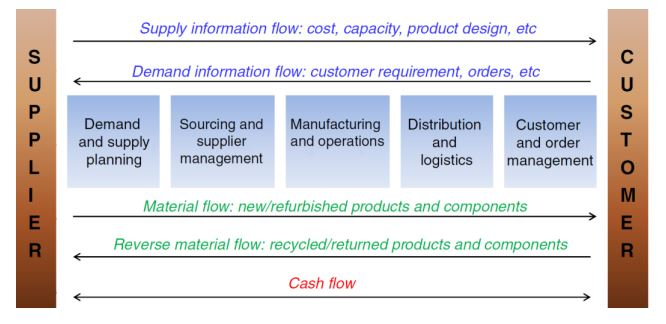
\includegraphics[width=.9\textwidth]{images/Alaa/supplyChain.JPG}%
     % you need to add the caption for the list of figures
    \caption[Supply chain process]{Supply chain process.}\label{fig: Supply chain process}%
  \end{figure}
  
While E-commerce includes online transactions business-to-business (B2B), business-to-consumer (B2C), consumer-to-business (C2B), and consumer-to-consumer (C2C), both with respect to virtual and physical goods, so it's dealing with the concept of delivery, to deliver the order to the requester. 

\section {Automating Delivery Process}
\hspace{2cm} Nowadays you can select and send your order to the market via software application and the delivery process will performed automatically, no need to go out from your room.
Autonomous vehicles are the next big thing in providing transportation solutions that are safer, cleaner and faster, so we can define autonomous vehicles as cars or trucks in which human drivers are never required to take control to safely operate the vehicle. Also known as “driverless” cars, they combine sensors and software to control, navigate, and drive the vehicle.\cite{web016}
\par
Automating delivery process helps to solve some problems and provides many benefits such as:
\begin{itemize}
    \item Providing safety and reducing car accidents and casualties immensely are benefits of automating the delivery process for the person who is delivering the orders.
    \item Making the delivery process as fast as possible to satisfy the client and save the customer's energy are benefits of automating the delivery process for the customer.
    \item provide paid salaries for drivers to be used on other things is one of benefits of automating the delivery process for the company.
    
\end{itemize}
While conventional delivery can increase the number of accidents as it is reported that 90 percent of car accidents are due to human error. In addition, conventional delivery process can take longer time until the order reaches to the requester, because the driver may be busy by making phone calls that will not only affect the delivery time but also will affect his safety.

\section{Use of Self-driving Cars in Delivery Systems}
\hspace{2cm} Self-driving car technology is advancing every day, and it's only a matter of time before fully driverless vehicles appear on public streets.
Almost daily, there's a new development in the driverless car space, and nearly every major car manufacturer, ride-sharing service and tech company from Apple to Google has bought into the driverless car industry. 
Self -driving car can be used in various and varied applications. The most common one is transferring someone from one place to another. It also can be used on indoor and outdoor delivery system to deliver items to the one who requested them. Now, we will consider some of the applications of self-driving car:
\par
\begin{itemize}
 \item\textbf{Apple self-driving cars}: Apple is actively testing its self-driving car tech, evidenced by several car sightings in the last few years. Though the vehicles lack proprietary markings, the cars are bedecked in all the gear needed to run self-driving systems and are often seen driving around Apple office buildings and into Apple complex parking lots. 
\par
Apple's self-driving cars are coming out of the shadows and onto public roads, but that's not all that's circulating about Apple's automotive project.
In May 2018, it was revealed by the California DMV that Apple's autonomous car permit now covers 55 cars and 83 drivers, giving it the second biggest autonomous car fleet in California.\cite{web029}
\begin{figure}[H]%
    \center%
    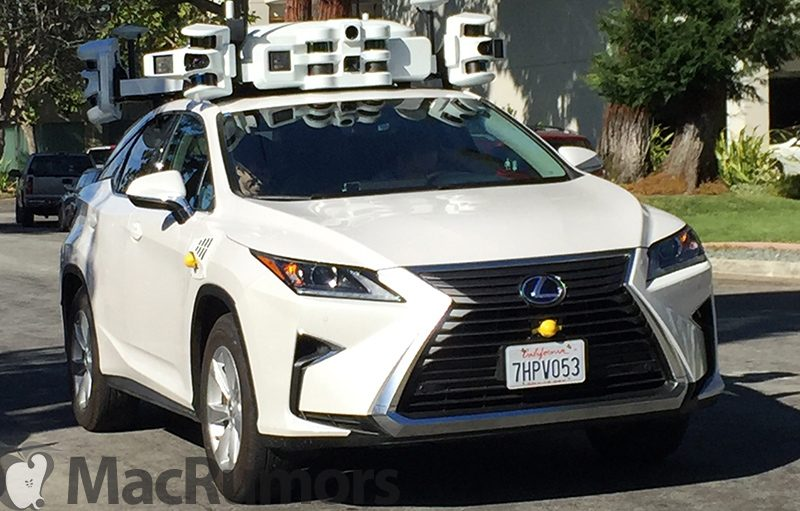
\includegraphics[width=.5\textwidth]{images/Alaa/apple.jpg}%
     % you need to add the caption for the list of figures
  \end{figure}
  
\item\textbf{Google's driverless cars }:
Waymo LLC is a self-driving technology development company. It is a subsidiary of Alphabet Inc. Waymo originated as a project of Google before it became a stand-alone subsidiary in December 2016. In April 2017, Waymo started a limited trial of a self-driving taxi service in Phoenix, Arizona. On December 5, 2018, the service launched a commercial self-driving car service called "Waymo One"; users in the Phoenix metropolitan area use an app to request a pick-up.\cite{web030}
\begin{figure}[H]%
    \center%
    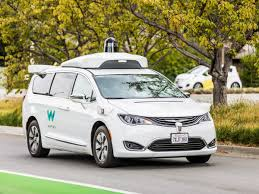
\includegraphics[width=.5\textwidth]{images/Alaa/waymo.jpg}%
     % you need to add the caption for the list of figures
  \end{figure}
  
\item\textbf{DoorDash delivery system }:
DoorDash announced it is partnering with General Motors' Cruise autonomous-vehicles unit to deliver food and groceries. The program will kick off early this year in the San Francisco area.
For now, a DoorDash delivery person will be present in the self-driving car and bring the groceries or meal to the doorstep. In the future, customers will be able to decide between picking up a delivery from the curb or via a fully autonomous delivery system.
The partnership is starting with one merchant and one vehicle, with plans to add more cars and merchants in the future.
Self-driving cars have been a growing presence in the food and grocery delivery business. Ford and Postmates announced plans to collaborate on a self-driving delivery service last June. Kroger partnered with robotics-company Nuro to deliver groceries in Scottsdale, Arizona. Domino's began testing self-driving cars in 2017.\cite{web031}

\par
\item\textbf{Olli car}: Olli is the world’s first self-driving, cognitive shuttle that uses IBM’s Watson technology to provide a more personalized experience. Olli is currently a “first mile/last mile” solution with the goal of being implemented in cities, towns and municipalities all over the world to solve congestion, pollution and accessibility issues. Olli currently would fill the service that a personal vehicle provides, allowing people to take Olli around town or from a transit station to their final destination.\cite{web032}

\begin{figure}[H]%
    \center%
    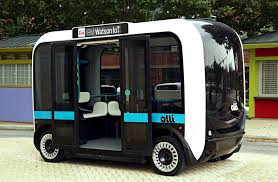
\includegraphics[width=.5\textwidth]{images/Alaa/olli.jpg}%
     % you need to add the caption for the list of figures
  \end{figure}
\end{itemize}


\section{History of Autonomous Delivery}
\hspace{2cm} Self-driving cars history dates back to the 1500s and has continued to this day. The chronological date of the self-driving cars will be shown since its inception:
\par
\begin{itemize}
\item \textbf{Da Vinci’s Self-Propelled Cart—c. 1500} Centuries before the invention of the automobile, Leonardo da Vinci designed a cart that could move without being pushed or pulled. Springs under high tension provided the power to the cart, and steering could be set in advance so the cart could move along a predetermined path. A distant precursor to the car, the device is sometimes considered the world’s first robot.

\par
\item \textbf{Whitehead Torpedo—1868} While these weapons of war emerged in the mid-1700s, Robert Whitehead’s invention of a torpedo that could propel itself underwater proved to be a game-changer for naval fleets around the world. The Whitehead torpedo could travel several hundred yards underwater and maintain depth, thanks to a pressurization system dubbed “The Secret.” Torpedo guidance would evolve dramatically thereafter and led to a wide range of weaponry, aircraft, and other autonomous devices.

\par
\item \textbf{Mechanical Mike Aircraft Autopilot—1933 } Extended travel times forced the development of autopilot systems for long-range aircraft. Mechanical Mike was a prototype autopilot designed by Sperry Gyroscope Co., and used by Wiley Post during a 13,000-mile, around-the-world flight in 1933. Gyroscopes kept track of the plane’s heading and interfaced with the controls to ensure accurate direction. Gyroscopes remain an integral part of autonomous vehicle tech today.

\par
\item \textbf{Teetor Cruise Control—1945} An engineer became so fed up with the rocking motion he experienced while riding in a car with his attorney behind the wheel that he developed one of the first cruise control system to smooth out the ride, using a mechanical throttle that could set the vehicle’s speed. The invention was commercialized in 1958.

\par
\item \textbf{Tsukuba Mechanical Engineering—1977 } As groundbreaking as the Stanford Cart was, it was still just a four-wheeled cart that looks more at home in the kitchen than on a roadway. Japan-based Tsukuba Mechanical produced an autonomous passenger vehicle that could recognize street markings while traveling at nearly 20 miles per hour, thanks to two vehicle-mounted cameras.

\par
\item \textbf{VaMoRs—1987} Another important step forward in autonomous tech came from German engineer Ernst Dickmanns, who equipped a sedan with a bank of cameras and 60 micro-processing modules to detect objects on the road—in front of and behind the vehicle.

\par
\item \textbf{General Atomics MQ-1 Predator—1995}  While we tend to think of autonomous vehicles as a means of converting humans from drivers to passengers, another class of autonomous devices are designed to travel completely alone. Nowhere is this more visible than in the world of drones, the most noteworthy of which has been General Atomics’ Predator, an unmanned plane that for 20 years has been piloting over global hotspots for 14 hours at a time. Drones aren’t just military vehicles, of course. The Predator is decked out with technologies being adapted for cars, including radar that can see through smoke or clouds and thermal imaging cameras that enable travel by night.

\par
\item \textbf{DARPA Challenges—2004-2013}  The U.S. Department of Defense’s research arm, DARPA, sponsored a series of challenges that pushed autonomous technologies forward. In 2004, a competition was held to challenge vehicles to self-navigate 150 miles of desert roadway. While no car completed the route, subsequent challenges have seen dramatic leaps in capabilities. The 2007 challenge simulated a 60-mile long urban environment, with four cars completing the route in the allotted six-hour time limit.

\par
\item \textbf{Tesla Autopilot—2015} The most significant aspect of Tesla’s semi-autonomous “Autopilot” feature, introduced in late 2015—which enabled hands-free control for highway and freeway driving— is that it was delivered in the form of a single software update to Model S owners overnight.\cite{web028}
\end{itemize}

\section{Related Products}
\hspace{2cm} Many companies generated self driving car and employed it in different applications, we will discuss some of them according to 2018 :
\par

\begin{itemize}
 \item \textbf{Nuro}: 
Nuro was founded by two former lead Google engineers, Dave Ferguson and Jiajun Zhu, who previously worked on the Google’s self-driving car project. They are designing a self-driving, small delivery vehicle which will travel on roads and focus on low-speed, local, and last-mile deliveries: groceries, laundry, packages or your take-out order. Rather than adapting existing vehicles designs to fit their model, their engineers have instead built something entirely new from scratch. Nuro’s first prototype has a “handle” on the roof which serves as a platform for the vehicle’s array of sensors — including LIDAR, cameras, and radars. Its self-driving status eliminates the need for all the normal inner components of a car — such as the steering wheel and driving seat — and means that the vehicle’s inner space can be dedicated solely to delivery lockers. Nuro is using a fleet of six self-driving cars to collect data and optimize routes, which will then be fed into its prototype vehicles. It has received a permit from the California DMV and plans to start testing on public roads later this year.\cite{web027}

\begin{figure}[H]%
    \center%
    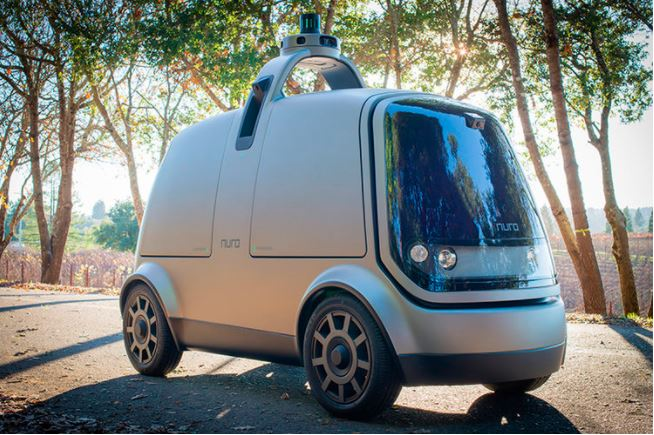
\includegraphics[width=.5\textwidth]{images/Alaa/nuro.JPG}%
  \end{figure}

\par
 \item \textbf{Robomart } : 
Robomart advertises itself as the ‘world’s first self-driving store’. Unlike other delivery services which focus on delivering goods pre-bought online, Robomart is quite literally a moving fresh produce store, bringing vegetables to people’s doors and allowing them to pick what they want on the spot. Similar to Uber and other taxi apps, customers tap a button to request the closest robomart circulating in their local area. Once it arrives, they head outside, unlock the doors, and shop for the products they want, closing the doors when they’re done and sending it on its way. \cite{web027} 

\begin{figure}[H]%
    \center%
    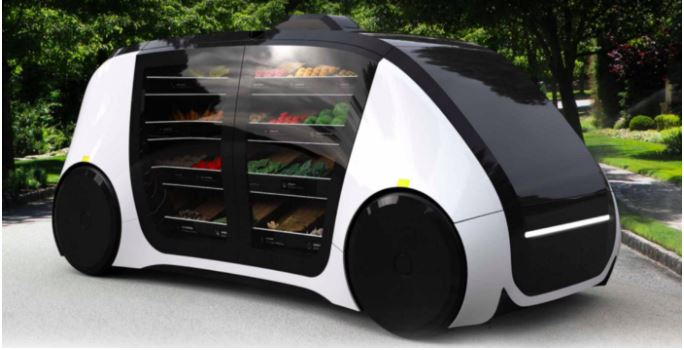
\includegraphics[width=.5\textwidth]{images/Alaa/robomart.JPG}%
  \end{figure}

\par
 \item \textbf{Delivery with Normal Autonomous cars} :
Nearly all major food delivery companies are playing with the idea of delivery through normal, autonomous vehicles. For example, Ford invested 1 billion dollar investment in artificial intelligence company Argo A.I. in 2017 and is now testing an autonomous pizza delivery vehicle in Miami in partnership with Domino’s. Toyota and Pizza Hut have also joined forces to ‘make pizza delivery more efficient’. \cite{web027}

\par
 \item \textbf{Gita }:
Gita is a round, mobile-carrier that follows people on the go; it was designed by PFF, a subsidiary of Piaggio Group that was created in 2015 to research and develop lightweight, intelligent mobility solutions for people and goods. Gita learns to navigate complex spaces by trailing its human owner and can carry up to 44 pounds of cargo and a volume of up to nearly 2,000 cubic inches (the equivalent of a case of wine, a loaded backpack, or two stuffed grocery bags). Gita is not therefore an autonomous delivery robot as such, but rather a kind of self-driving ‘moving bag’, that helps those with a mobile lifestyle — from millennials and parents to seniors and disabled individuals — to carry more than they could on their own.\cite{web027}
\begin{figure}[H]%
    \center%
    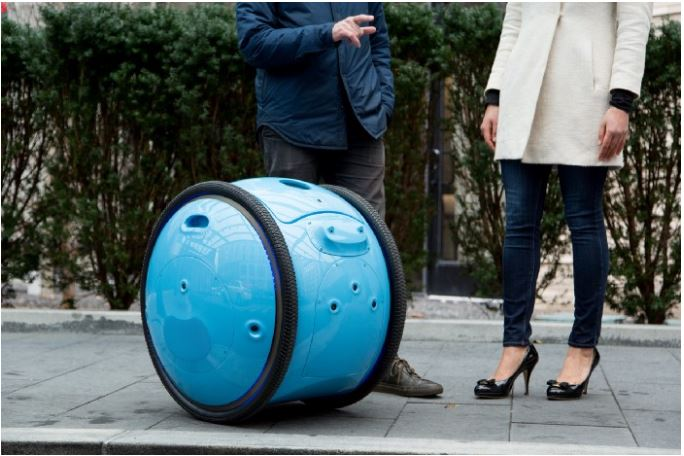
\includegraphics[width=.5\textwidth]{images/Alaa/gita.JPG}%
  \end{figure}


\par
 \item \textbf{Amazon Prime Air}:
Amazon Prime Air is a delivery system developed by Amazon that is designed to safely deliver packages to customers using unmanned aerial vehicles (a.k.a, drones). Customers choose from a selection of items in an Amazon fulfilment centre near their homes and just moments after they order, an Amazon drone makes it way down an automated track and lifts off into the open sky, heading to its destination completely on its own. Travelling at a height of roughly 400ft, carrying packages up 5 pounds, guided by GPS and using so-called ‘sense-and-avoid’ technologies, these drones deliver packages in under 30 minutes. \cite{web027}
\begin{figure}[H]%
    \center%
    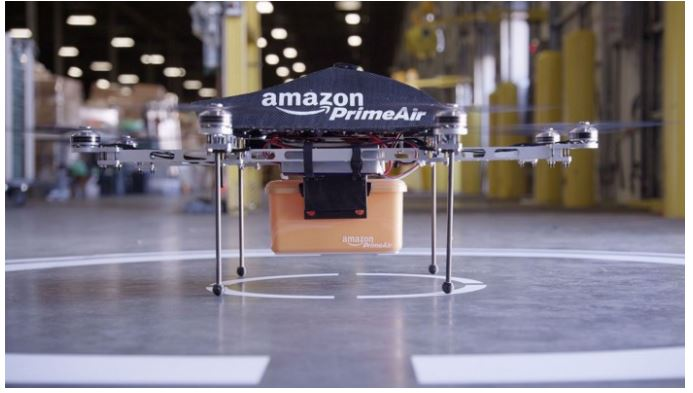
\includegraphics[width=.5\textwidth]{images/Alaa/prime.JPG}%
  \end{figure}
\end{itemize}

\section{Project Scope}
\hspace{2cm} Last mile delivery is an important term in the communities of supply chain management and e-commerce. It refers to transferring goods and materials from a transportation hub to their final destinations at homes. In this project we propose a fully autonomous robotic system for last mile delivery applications. The proposed system is supposed to perform two main functions. The first function is connecting clients purchasing different objects with the vendors supplying these objects in a certain area. The second function is transferring purchased objects to their final destinations. We aim to develop a self-driving robot that is capable of safely transferring objects in noisy and crowded outdoor environments.

Our work to complete this project is divided into three milestones:
 \begin{itemize}
\item   Build a self-driving robot which is supposed to perform the following tasks:
    \begin{itemize}
    \item Low level motion control.
    \item Obstacle avoidance during motion.
    \item Path tracking to reach destination.
    \item Localization
    \item Sensor Fusion using sensors besides robot odometry to increase accuracy of localization process.
    \end{itemize}
\item  Develop a web server to perform the following tasks:
    \begin{itemize}
    \item Monitor all the robots in the system.
    \item Keep track of vendors using our service and their products.
    \item Path planning to determine the way for robots.
    \end{itemize}
\item  Design a suitable user interface for vendors, who use our service to transfer their products to purchasers, and clients shipping their groceries through our service.

\end{itemize}

%%%%%%%%%%%%%%%%%%%%%%%%%%%%%%%%%%%%%%%%%%%%%%%%%%%%%%%%%%%%%%%%%%%%%%%%%%%%%%%%%%%%%%%%%%%%%%%%%%%%%%%%%%%%%%%%%%